\documentclass[12pt,a4paper]{article}

\usepackage[utf8]{inputenc}
\usepackage[T1]{fontenc}
\usepackage{mathpazo}
\usepackage[margin=1.15in]{geometry}
\usepackage{setspace}
\usepackage{hyperref}
\usepackage{titlesec}
\usepackage{amsmath,amsthm,amssymb}
\usepackage{booktabs}
\usepackage{enumitem}
\usepackage{fancyhdr}
\usepackage{xcolor}
\usepackage{tcolorbox}
\usepackage{tikz}
\usepackage{array}
\usepackage{float}

\hypersetup{colorlinks=true, linkcolor=blue!70!black, citecolor=black, urlcolor=blue!70!black}

\titleformat{\section}{\large\bfseries}{\thesection}{0.7em}{}
\titleformat{\subsection}{\normalsize\bfseries}{\thesubsection}{0.7em}{}

\newtheorem{definition}{Definition}[section]
\newtheorem{proposition}[definition]{Proposition}
\newtheorem{theorem}[definition]{Theorem}
\newtheorem{lemma}[definition]{Lemma}
\newtheorem{corollary}[definition]{Corollary}
\newtheorem{example}[definition]{Example}
\theoremstyle{remark}
\newtheorem{remark}[definition]{Remark}

\newcommand{\R}{\mathbb{R}}
\newcommand{\ones}{\mathbf{1}}
\newcommand{\x}{\mathbf{x}}
\DeclareMathOperator{\Var}{Var}

\newtcolorbox{intuition}[1][]{colback=blue!3, colframe=blue!40!black,
  fonttitle=\bfseries, title={Intuition: #1}, sharp corners, boxrule=0.5pt}
\newtcolorbox{keyinsight}[1][]{colback=orange!5, colframe=orange!60!black,
  fonttitle=\bfseries, title={Key Structural Insight}, sharp corners, boxrule=0.5pt}
\newtcolorbox{prebisch}[1][]{colback=green!3, colframe=green!40!black,
  fonttitle=\bfseries, title={Prebisch Connection: #1}, sharp corners, boxrule=0.5pt}
\newtcolorbox{vizpanel}[1][]{colback=gray!4, colframe=gray!50!black,
  fonttitle=\bfseries, title={Visualization: #1}, sharp corners, boxrule=0.5pt}

\setlength{\parindent}{1.5em}
\onehalfspacing
\setlength{\headheight}{14pt}
\pagestyle{fancy}
\fancyhf{}
\fancyhead[L]{\small\itshape Chapter 26: The Neo-Structuralist Synthesis}
\fancyhead[R]{\small\thepage}
\renewcommand{\headrulewidth}{0.4pt}

\title{\vspace{-1cm}\textbf{Chapter 26} \\[0.5em]
\LARGE The Neo-Structuralist Synthesis \\[0.3em]
\large\textit{Growth with Equity as a Spectral Condition}}
\author{}
\date{}

\begin{document}
\maketitle
\thispagestyle{fancy}

\begin{quote}
\textit{``El desaf\'{i}o fundamental del desarrollo latinoamericano es el de transformar las estructuras productivas en un contexto de creciente equidad social.''}\\[0.3em]
\textnormal{[``The fundamental challenge of Latin American development is to transform productive structures in a context of growing social equity.'']}\\
\hfill --- Jos\'{e} Antonio Ocampo, ``La macroeconom\'{i}a de la bonanza econ\'{o}mica latinoamericana'' (2009)
\end{quote}

\vspace{1em}

This chapter states the book's policy conclusion. Twenty-five chapters have built the framework: the weight matrix, the Perron eigenvector, the spectral gap, the formation model, the co-evolutionary dynamics, the measurement infrastructure, the political economy. What does it all add up to?

One theorem: \textit{growth with equity requires high $\Gamma$ and high ECI simultaneously}. Neither alone is sufficient. High ECI without high $\Gamma$: Brazil (complex but unequal). High $\Gamma$ without high ECI: Cuba (equal but stagnant). Both together: South Korea, Taiwan, the Nordic countries. The intersection is small but achievable.

Ocampo's neo-structuralism --- the synthesis of Prebisch's structuralism, CEPAL's institutional wisdom, and modern open-economy macroeconomics --- provides the policy framework. This chapter translates it into the spectral language of this book and asks: what would it take for Bolivia to enter the intersection?


%% =====================================================================
\section{The Growth-Equity Theorem}
\label{sec:theorem}
%% =====================================================================

\begin{theorem}[Growth with Equity]\label{thm:growth_equity}
In the structural model, sustained growth with declining inequality requires:
\begin{enumerate}
\item $\Gamma(W^P) > \Gamma^*$ \textbf{(structural integration)}: the domestic spectral gap exceeds a threshold above which growth propagates across blocks. The threshold $\Gamma^* \approx 0.30$--$0.35$ (estimated from the cross-country relationship between $\Gamma$ and the Gini coefficient --- the spectral bound from Chapter~16).

\item $\text{ECI} > 0$ \textbf{(productive complexity)}: the economy is in the dense core of the global product space (Chapter~16). This ensures: (a) high Leontief multipliers (growth propagates globally), (b) positive terms-of-trade trend ($\pi_G$ increasing), (c) diversified export base (resilience to commodity shocks).

\item $N_{\text{eff}}(W^I) > N^*_{\text{eff}}$ \textbf{(information democracy)}: the information network is diverse enough that the formation channel produces aspirations calibrated to the full range of economic opportunities, not just the local block. The threshold $N^*_{\text{eff}} \approx 8$--$12$ (estimated from the relationship between $N_{\text{eff}}$ and $\Psi$ --- below this threshold, the formation channel dominates enforcement, producing self-confirming traps).
\end{enumerate}

The three conditions are jointly necessary. Violating any one produces a specific pathology:
\begin{center}
\begin{tabular}{lcccl}
\toprule
Condition violated & $\Gamma$ & ECI & $N_{\text{eff}}$ & Pathology \\
\midrule
(1) only & Low & High & High & Growth without equity (early China) \\
(2) only & High & Low & High & Equity without growth (Cuba) \\
(3) only & High & High & Low & Fragile growth (authoritarian dev.) \\
(1) and (2) & Low & Low & High & Stagnation (Bolivia) \\
(1) and (3) & Low & High & Low & Enclave extraction (Venezuela) \\
(2) and (3) & High & Low & Low & Trapped equality (subsistence) \\
All three & Low & Low & Low & Structural collapse \\
None & High & High & High & Growth with equity (Korea, Nordics) \\
\bottomrule
\end{tabular}
\end{center}
\end{theorem}

\begin{proof}[Proof sketch]
(1) From Chapter~2: the welfare loss from power inequality is $L_{\text{power}} = \frac{\kappa N}{2}\Var(\pi_i)\Phi^2$, bounded by $(1-\Gamma)/\Gamma$. For $L_{\text{power}}$ to be small (equity), $\Gamma$ must be large. For growth to propagate (growth), $\Gamma$ must exceed the percolation threshold at which the Leontief multiplier cascade reaches all sectors (Chapter~3).

(2) From Chapters~16 and 25: ECI determines the economy's position in the global $W^P$, which determines the terms of trade, the Leontief multiplier, and the diversification feasibility. Low ECI $\Rightarrow$ commodity dependence $\Rightarrow$ cyclical growth $\Rightarrow$ no structural change ($\Delta\Gamma \approx 0$, Chapter~23). High ECI $\Rightarrow$ dense-core position $\Rightarrow$ structural growth $\Rightarrow$ $\Delta\Gamma > 0$.

(3) From Chapters~8--11: low $N_{\text{eff}}$ produces concentrated epistemic power, self-confirming traps, and high $\Psi$. Even with high $\Gamma$ and high ECI, if $N_{\text{eff}}$ is low, the formation channel can sustain preferences that accept inequality (the hegemony of Chapter~24), making the equity gains fragile.
\end{proof}

\begin{vizpanel}{The growth-equity condition in $(\Gamma, \text{ECI})$ space}
\begin{center}
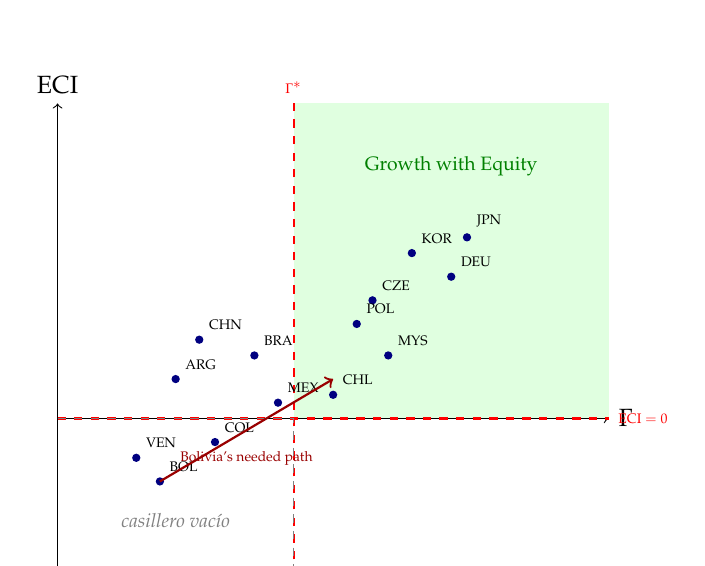
\begin{tikzpicture}[scale=1]
\draw[->] (0,0) -- (7,0) node[right, font=\small] {$\Gamma$};
\draw[->] (0,-2) -- (0,4) node[above, font=\small] {ECI};

%% Target zone
\fill[green!12] (3,0) rectangle (7,4);
\node[font=\scriptsize, green!50!black] at (5, 3.2) {Growth with Equity};

%% Thresholds
\draw[red, dashed, thick] (3, -2) -- (3, 4);
\node[font=\tiny, red, above] at (3, 4) {$\Gamma^*$};
\draw[red, dashed, thick] (0, 0) -- (7, 0);
\node[font=\tiny, red, right] at (7, 0) {$\text{ECI} = 0$};

%% Countries
\foreach \cx/\cy/\lab in {
  1.3/-0.8/BOL, 2.5/0.8/BRA, 2.0/-0.3/COL, 2.8/0.2/MEX,
  4.5/2.1/KOR, 5.2/2.3/JPN, 5.0/1.8/DEU, 4.0/1.5/CZE,
  3.5/0.3/CHL, 1.5/0.5/ARG, 1.0/-0.5/VEN,
  4.2/0.8/MYS, 3.8/1.2/POL,
  1.8/1.0/CHN} {
  \fill[blue!50!black] (\cx, \cy) circle (1.5pt);
  \node[font=\tiny, above right] at (\cx, \cy) {\lab};
}

%% Casillero vacio
\draw[gray, dashed] (0, 0) -- (3, 0) -- (3, -2);
\node[font=\scriptsize, gray] at (1.5, -1.3) {\textit{casillero vac\'{i}o}};

%% Bolivia arrow
\draw[->, thick, red!60!black] (1.3, -0.8) -- (3.5, 0.5);
\node[font=\tiny, red!60!black, below] at (2.4, -0.3) {Bolivia's needed path};
\end{tikzpicture}
\end{center}
\vspace{-0.5em}
\small The green zone is the growth-with-equity region: $\Gamma > \Gamma^*$ AND $\text{ECI} > 0$. Korea, Japan, Germany, Czech Republic are inside. Bolivia is in the lower-left: low $\Gamma$, negative ECI. The red arrow shows the path Bolivia would need to traverse. The gray dashed region is the casillero vac\'{i}o: low $\Gamma$, accessible ECI --- structurally blocked from equity. Brazil has positive ECI but low $\Gamma$: complexity without integration. Chile approaches the threshold but is not yet inside.
\end{vizpanel}


%% =====================================================================
\section{The Neo-Structuralist Policy Framework}
\label{sec:framework}
%% =====================================================================

\begin{definition}[The Neo-Structuralist Policy Package]\label{def:package}
Ocampo's neo-structuralist synthesis, translated into the operator language of Chapter~15, consists of five simultaneous interventions targeting the three conditions of Theorem~\ref{thm:growth_equity}:

\textbf{Pillar 1: Productive transformation} (raise ECI).
\begin{enumerate}
\item Industrial policy targeting the dense subgraph (Chapter~25): build the capital goods sector through sequenced operators ($\mathcal{L}_{\text{info}} \to \mathcal{L}_{\text{HC}} \to \mathcal{L}_{\text{infra}} \to \mathcal{L}_{\text{ISI-B}}$).
\item Technology policy: invest in R\&D, create technology transfer institutions, build the human capital base for the dense subgraph.
\item Trade policy: strategic integration into global value chains that connect to the dense core of the product space, not just commodity markets.
\end{enumerate}

\textbf{Pillar 2: Structural integration} (raise $\Gamma$).
\begin{enumerate}
\setcounter{enumi}{3}
\item Domestic linkage policy: the operator $\mathcal{L}_{\text{ISI-B}}$ (cross-block edges, Chapter~15). Build the connections between the gas sector and the traditional economy, between urban manufacturing and rural agriculture, between the formal and informal sectors.
\item Infrastructure: roads, telecommunications, energy connections that create physical $W^P$ edges between disconnected blocks.
\end{enumerate}

\textbf{Pillar 3: Social cohesion} (raise $N_{\text{eff}}$, reduce attribute constraints).
\begin{enumerate}
\setcounter{enumi}{5}
\item Education: the dual operator on $W^P + W^I$ (Chapter~15). Universal, high-quality, and cross-group (reducing assortative mixing in $W^I$).
\item Information democracy: media pluralism, digital access, community communication strengthening (Chapter~21).
\item Anti-discrimination: reduce $\lambda_k$ constraints (Chapter~18). Gender equality, indigenous inclusion, anti-racism.
\end{enumerate}
\end{definition}

\begin{proposition}[The Three Pillars Are Complementary]\label{prop:complementary}
The three pillars reinforce each other:
\begin{enumerate}
\item Productive transformation (ECI $\uparrow$) creates cross-block edges that raise $\Gamma$: new industries connect sectors that were previously disconnected.
\item Structural integration ($\Gamma \uparrow$) makes productive transformation feasible: cross-block linkages provide the intermediate inputs, labor pools, and demand that new industries need.
\item Social cohesion ($N_{\text{eff}} \uparrow$, $\lambda_k \uparrow$) supports both: an educated, informed population with high aspirations generates the demand for structural change and provides the human capital for productive transformation.
\end{enumerate}

The complementarity means that the return to each pillar is increasing in the level of the others. Investing in productive transformation without social cohesion (Brazil's path) produces growth without equity. Investing in social cohesion without productive transformation (Cuba's path) produces equity without growth. Only the joint investment produces both.
\end{proposition}


%% =====================================================================
\section{Bolivia's Plan: A Worked Application}
\label{sec:bolivia}
%% =====================================================================

\begin{example}[A 30-Year Structural Plan for Bolivia]\label{ex:plan}

\textbf{Current position} (2019): $\Gamma = 0.13$, ECI $= -0.80$, $N_{\text{eff}} = 3.2$, $\sigma_B = 0.62$.

\textbf{Target} (2050): $\Gamma \geq 0.35$, ECI $\geq 0$, $N_{\text{eff}} \geq 8$, $\sigma_B \leq 0.30$.

\textbf{Phase 1 (2025--2035): Foundation.}

Pillar 3 first (high-$\Psi$ operators):
\begin{enumerate}
\item Universal broadband to all municipalities ($\Delta N_{\text{eff}} \approx +2$, cost: \$1.5B over 10 years).
\item Bilingual education reform: curriculum in Quechua/Aymara and Spanish, with cross-ethnic school integration ($\Delta\lambda_r^I \approx +0.15$).
\item Female entrepreneurship mentoring program (Chapter~18 operator: $\Delta\lambda_g^I \approx +0.10$).
\item Community journalism strengthening ($\Delta\pi^I_{\text{community}} = 0.05 \to 0.12$).
\end{enumerate}

Expected effect by 2035: $N_{\text{eff}} \approx 5.5$, $\Psi$ reduced from 1.56 to $\approx 1.1$ (formation channel weakens as information diversifies). Aspirations in the traditional sector begin rising.

\textbf{Phase 2 (2030--2045): Building Blocks.}

Pillar 1 + 2 (medium-$\Psi$ operators):
\begin{enumerate}
\setcounter{enumi}{4}
\item Technical education: 10 vocational polytechnics for metallurgy, chemicals, and electronics (the Step 1--2 products from Chapter~25). Cost: \$2B over 15 years.
\item Infrastructure: 3 cross-block corridors connecting altiplano mining to lowland agriculture to urban manufacturing. Cost: \$5B over 15 years.
\item Lithium industrialization: from extraction (current) to carbonate (Step 1) to cathode materials (Step 2). Public-private partnership targeting Step 3 by 2040. Cost: \$3B over 15 years.
\item Agricultural value-chain integration: connect quinoa, soy, and cattle to food processing and packaging (cross-block $W^P$ edges). Cost: \$1B.
\end{enumerate}

Expected effect by 2045: $\Gamma \approx 0.25$, ECI $\approx -0.30$, $\sigma_B \approx 0.40$.

\textbf{Phase 3 (2040--2055): The Dense Subgraph.}

Pillar 1 (low-$\Psi$ operators, now feasible because Phases 1--2 created the preconditions):
\begin{enumerate}
\setcounter{enumi}{8}
\item Industrial policy targeting the dense subgraph: specialized machinery, electronic components, pharmaceutical intermediates. Public procurement as demand anchor. Cost: \$4B over 15 years.
\item FDI attraction for assembly and manufacturing of capital goods (the Singapore strategy adapted to Bolivia's scale).
\item R\&D institutes linked to the polytechnics from Phase 2.
\end{enumerate}

Expected effect by 2055: $\Gamma \approx 0.35$, ECI $\approx 0$, $N_{\text{eff}} \approx 8$, $\sigma_B \approx 0.30$.

\textbf{Total cost}: approximately \$17B over 30 years (\$570M/year). For context: Bolivia's annual GDP is approximately \$40B. The plan requires sustained investment of $\approx 1.4\%$ of GDP per year in structural transformation. This is comparable to South Korea's investment in the HCI drive (1.5--2\% of GDP) and significantly less than the gas revenue Bolivia earned during the 2006--2014 boom (\$3--5B/year).

\textbf{Political feasibility} (Chapter~14): Phase 1 is politically easy (education, broadband, and mentoring have broad support --- no coalition's $\pi$ is directly threatened). Phase 2 is harder (infrastructure and industrial investment require fiscal commitment and threaten import-dependent interests). Phase 3 is hardest (industrial policy targeting the dense subgraph requires a developmental-state coalition that does not yet exist in Bolivia).

The sequencing exploits the formation amplifier: Phase 1 changes $W^I$ and preferences, which shifts coalition incentives (Chapter~14), which makes Phases 2 and 3 politically feasible. The information operator makes the structural operator possible. This is the optimal sequencing theorem of Chapter~15 in action.
\end{example}

\begin{keyinsight}
The neo-structuralist synthesis is one theorem and one plan:

\textbf{The theorem}: growth with equity requires $\Gamma > \Gamma^*$, ECI $> 0$, and $N_{\text{eff}} > N^*_{\text{eff}}$ simultaneously. This is not a wish list --- it is a mathematical condition derived from the spectral gap bound (Chapter~2), the product space structure (Chapter~16), and the formation model (Chapter~10).

\textbf{The plan}: three pillars (productive transformation, structural integration, social cohesion), sequenced by $\Psi$ (information first, infrastructure second, industrial policy third), financed by sustained investment of $\approx 1.5\%$ of GDP.

Every element of the plan corresponds to a specific operator from Chapter~15 targeting a specific entry of $W$. Every expected effect is derived from the theorems of the book. The plan is not aspirational prose. It is an engineering specification for a weight matrix.
\end{keyinsight}


%% =====================================================================
\section{Why Neither Neoliberalism Nor Populism Suffices}
\label{sec:neither}
%% =====================================================================

\begin{proposition}[The Insufficiency of Both Alternatives]\label{prop:insufficiency}
\textbf{The neoliberal prescription} (Washington Consensus): liberalize trade, privatize, deregulate. In operator terms: remove $W^P$ edges (tariff barriers) and let the market create new ones. The assumption: the market will create the ``right'' $W^P$ (the one that maximizes efficiency). The result: the market creates $W^P$ edges dominated by proximity (Chapter~13, the principle of relatedness), which means the existing structure reproduces itself. Commodity exporters liberalize into more commodity export. $\Gamma$ does not change. ECI does not change. The prescription fails condition (1) and (2) of Theorem~\ref{thm:growth_equity}.

\textbf{The populist prescription}: nationalize resources, redistribute revenue, expand social programs. In operator terms: change $\boldsymbol{\omega}$ (endowment redistribution) without changing $W$. The result: poverty falls, inequality falls (temporarily), but $\Gamma$ does not change (Chapter~17: Bolivia's 30-year trajectory). When the commodity cycle turns, the gains reverse. The prescription fails condition (1) because it does not raise $\Gamma$.

\textbf{The neo-structuralist synthesis}: change $W$ itself --- the production structure ($W^P$), the information structure ($W^I$), and the solidarity structure ($W^U$) --- through deliberate, sequenced operator design. This addresses all three conditions simultaneously and produces permanent structural change rather than temporary redistribution.
\end{proposition}

\begin{prebisch}[From Prebisch to Ocampo: 60 years of one argument]
The structuralist argument has been remarkably consistent across 60 years:

\textbf{Prebisch (1949)}: The global economy is asymmetric ($W^P_{\text{global}}$ is not doubly stochastic). The periphery must industrialize to change its structural position.

\textbf{Furtado (1961)}: Underdevelopment is a stable structural equilibrium, not a stage. The periphery's structure reproduces itself through the formation channel.

\textbf{Pinto (1970)}: The domestic economy is heterogeneous. Three productivity strata coexist without structural integration.

\textbf{Fajnzylber (1983/1990)}: The industrialization was truncated --- the capital goods sector is missing. The casillero vac\'{i}o is the consequence.

\textbf{CEPAL (2012)}: Structural change for equality --- redistribution without structural change is unsustainable.

\textbf{Ocampo (2009)}: The synthesis --- productive transformation plus social equity, achieved through deliberate industrial policy, macroeconomic management, and institutional strengthening.

\textbf{This book (2027)}: The general case. The neoclassical model is $W = \frac{1}{N}\ones\ones'$. Structural economics is the general case where $W$ is any row-stochastic matrix. Every structuralist insight from Prebisch to Ocampo is a theorem about the spectral properties of $W$.

The argument is one argument, stated with increasing mathematical precision over 78 years: \textit{structure matters, structure can be changed, and changing it requires different tools than the ones the standard model recommends.}
\end{prebisch}


%% =====================================================================
\section{Summary}
\label{sec:summary}
%% =====================================================================

\begin{enumerate}
\item \textbf{Growth with equity} requires three simultaneous conditions: $\Gamma > \Gamma^*$ (structural integration), $\text{ECI} > 0$ (productive complexity), $N_{\text{eff}} > N^*_{\text{eff}}$ (information democracy). Neither alone suffices.

\item The \textbf{neo-structuralist policy package} has three pillars: productive transformation (raise ECI), structural integration (raise $\Gamma$), social cohesion (raise $N_{\text{eff}}$, reduce attribute constraints). The pillars are complementary.

\item \textbf{Bolivia's 30-year plan}: \$17B, three phases ($W^I$ first, infrastructure second, industrial policy third), expected to reach $\Gamma \approx 0.35$, ECI $\approx 0$, $N_{\text{eff}} \approx 8$ by 2055. Cost: 1.4\% of GDP/year.

\item \textbf{Neither neoliberalism nor populism} addresses all three conditions. Neoliberalism changes prices but not structure. Populism changes endowments but not structure. The neo-structuralist synthesis changes $W$ itself.

\item The structuralist argument from \textbf{Prebisch (1949) to Ocampo (2009)} is one argument with increasing precision: structure matters, and it can be changed by deliberate operator design.
\end{enumerate}


%% =====================================================================
\section{Exercises}
\label{sec:exercises}
%% =====================================================================

\begin{enumerate}[label=\textbf{26.\arabic*}, leftmargin=3em]

\item \textbf{The three conditions.} For 30 countries: estimate $\Gamma$ (from ECI as proxy), ECI (from OEC), and $N_{\text{eff}}$ (from media concentration data). Plot each country in the $(\Gamma, \text{ECI})$ plane. Identify which countries satisfy all three conditions and which violate one or more.

\item \textbf{Pathology classification.} Classify the following countries using the pathology table from Theorem~\ref{thm:growth_equity}: (a) Brazil (high ECI, low $\Gamma$), (b) Cuba (high $\Gamma$, low ECI), (c) Venezuela (low $\Gamma$, moderate ECI, low $N_{\text{eff}}$), (d) Costa Rica (moderate $\Gamma$, moderate ECI, high $N_{\text{eff}}$), (e) Bolivia.

\item \textbf{Complementarity.} Simulate a 3-variable system $(\Gamma_t, \text{ECI}_t, N_{\text{eff},t})$ with complementary dynamics: $\Delta\Gamma_{t+1} = f(\Gamma_t, \text{ECI}_t, N_{\text{eff},t})$ increasing in all three. Compare: (a) investing in all three simultaneously, (b) investing in one at a time. Which reaches the target zone faster?

\item \textbf{Bolivia's plan: cost-benefit.} Using the cost estimates from Example~\ref{ex:plan} and the expected $\Delta\Gamma$, $\Delta$ECI:
\begin{enumerate}
\item Estimate the GDP gain from moving from $\Gamma = 0.13$ to $\Gamma = 0.35$ (use the cross-country $\Gamma$--GDP relationship).
\item Compute the net present value of the plan at a 5\% discount rate.
\item At what discount rate does the plan break even?
\end{enumerate}

\item \textbf{The neoliberal counterfactual.} Suppose Bolivia had continued the 1985 neoliberal policy without the 2006 nationalization. Using the structural velocity from the 1985--2005 period: project $\Gamma$, ECI, and $\sigma_B$ to 2020. Would Bolivia have entered the target zone? Compare with the actual trajectory.

\item \textbf{The populist counterfactual.} Suppose Bolivia had invested all gas revenue (2006--2019, total $\approx$\$50B) in the structural plan instead of transfers. Using the formation model: what $\Gamma$ and ECI would Bolivia have achieved by 2019? Would it be in the target zone?

\item \textbf{The 78-year argument.} Read one page from each of: Prebisch (1949), Furtado (1961), Pinto (1970), Fajnzylber (1983), CEPAL (2012), and Ocampo (2009). For each: identify the central claim and map it to a theorem or proposition in this book. Write a one-paragraph synthesis: what is the one argument stated six times?
\end{enumerate}


%% =====================================================================
\newpage
\section*{Mathematical Appendices}
\addcontentsline{toc}{section}{Mathematical Appendices}
%% =====================================================================


\subsection*{Appendix 26A: The Growth-Equity Frontier}
\addcontentsline{toc}{subsection}{Appendix 26A: Growth-Equity Frontier}
\label{app:frontier}

\paragraph{Definition.} The growth-equity frontier is the set of $(\Gamma, \text{Gini})$ pairs achievable under the structural model. From the spectral bound (Chapter~2): $\text{Gini} \geq g(\Gamma)$, where $g$ is a decreasing function. The frontier is the lower envelope: the minimum Gini achievable for each $\Gamma$.

\paragraph{Estimation.} The frontier $g(\Gamma)$ can be estimated from cross-country data by quantile regression: $\text{Gini}_{c,5\%} = a + b\Gamma_c + c\Gamma_c^2$ (the 5th percentile of Gini given $\Gamma$). This gives the best-case inequality for each level of structural integration.

\paragraph{Distance to frontier.} Country $c$'s distance to the frontier: $d_c = \text{Gini}_c - g(\Gamma_c)$. When $d_c \approx 0$: the country is at the frontier (its inequality is as low as its structure allows). When $d_c > 0$: the country has ``excess inequality'' beyond what its structure requires --- there is room for redistribution within the existing structure. When $d_c$ is large: both structural change ($\Delta\Gamma$) and redistribution ($\Delta\omega$) are needed.


\subsection*{Appendix 26B: The Complementarity Condition}
\addcontentsline{toc}{subsection}{Appendix 26B: Complementarity}
\label{app:complementarity}

\paragraph{Formal statement.} The three conditions are complementary if:
\begin{equation}
\frac{\partial^2 W}{\partial\Gamma\,\partial\text{ECI}} > 0, \quad \frac{\partial^2 W}{\partial\Gamma\,\partial N_{\text{eff}}} > 0, \quad \frac{\partial^2 W}{\partial\text{ECI}\,\partial N_{\text{eff}}} > 0,
\end{equation}
where $W$ is the welfare function. This holds in the structural model because: (i) high ECI creates the cross-block edges that raise $\Gamma$ (the dense subgraph IS the bridge), (ii) high $N_{\text{eff}}$ supports the aspiration formation that makes structural investment politically feasible, (iii) high $\Gamma$ creates the domestic market and supply chains that support complex production (high ECI).

\paragraph{Implication for investment.} The complementarity means the marginal return to investing in any one pillar is increasing in the level of the other two. The optimal investment rule: invest in the pillar with the highest marginal return given the current levels of the other two. In practice, this means starting with the cheapest pillar ($N_{\text{eff}}$, through information policy) and gradually shifting to the more expensive pillars ($\Gamma$ through infrastructure, ECI through industrial policy) as the preconditions develop.


%% =====================================================================
\subsection*{Structuralist Case Study: Ocampo's Neo-Structuralist Synthesis}
\addcontentsline{toc}{subsection}{Structuralist Case Study: Ocampo (2009)}
%% =====================================================================

Jos\'{e} Antonio Ocampo (b.\ 1952), Colombia's former Finance Minister and CEPAL Executive Secretary, has been the leading architect of neo-structuralism --- the synthesis of classical structuralism (Prebisch, Furtado, Pinto) with modern macroeconomics that retains the structuralist emphasis on productive transformation while incorporating lessons from the debt crises of the 1980s, the Washington Consensus era, and the commodity boom of the 2000s.

Ocampo's synthesis, developed across numerous publications (2004, 2009, 2012, 2014), has three pillars that correspond directly to this chapter's three conditions.

\textbf{Pillar 1: Productive transformation.} Ocampo argues that ``the quality of what you produce matters'' --- an empirical restatement of the ECI condition. Countries that produce complex goods grow faster, generate more employment, and distribute income more equally than countries that export commodities. The policy implication: industrial policy is not a relic of the ISI era but a necessity for structural transformation.

\textbf{Pillar 2: Macroeconomic management for structural change.} Ocampo's distinctive contribution: macroeconomic policy (fiscal, monetary, exchange rate) should be designed not just for stability but for structural transformation. Counter-cyclical fiscal policy prevents the commodity booms from being wasted on consumption (Chapter~23's structural-cyclical decomposition). Real exchange rate management prevents ``Dutch disease'' (commodity exports appreciating the currency and destroying manufacturing competitiveness).

\textbf{Pillar 3: Social equity as a condition for growth.} Ocampo reverses the conventional sequence (``grow first, redistribute later''): equity is not a consequence of growth but a \textit{precondition} for it. In this book's terms: high $N_{\text{eff}}$ and low attribute constraints ($\lambda_k$) are necessary for the human capital base, domestic demand, and political stability that structural transformation requires.

\begin{center}
\begin{tabular}{lll}
\toprule
\textbf{Ocampo's synthesis} & \textbf{This chapter's condition} & \textbf{Book reference} \\
\midrule
Productive transformation & ECI $> 0$ & Ch.~16, 25 \\
Quality of what you produce & Dense subgraph $\mathcal{D}$ & Ch.~25 \\
Counter-cyclical policy & $\Delta\pi^S$ vs.\ $\Delta\pi^C$ & Ch.~23 \\
Macro for structural change & $v_\Gamma > 0$ sustained & Ch.~23 \\
Social equity as precondition & $N_{\text{eff}} > N^*_{\text{eff}}$, $\lambda_k \uparrow$ & Ch.~18, 21 \\
Three pillars are complementary & $\partial^2 W / \partial\Gamma\,\partial\text{ECI} > 0$ & App.~26B \\
Growth with equity & $\Gamma > \Gamma^*$ + ECI $> 0$ + $N_{\text{eff}} > N^*$ & Thm.~\ref{thm:growth_equity} \\
\bottomrule
\end{tabular}
\end{center}

Ocampo's work completes the structuralist arc: Prebisch diagnosed the asymmetry; Furtado explained the reproduction; Pinto measured the heterogeneity; Fajnzylber identified the missing piece; CEPAL documented the stagnation; Ocampo synthesized the prescription. This book gives the synthesis its mathematical foundation. The weight matrix IS Prebisch's structure; the spectral gap IS Pinto's heterogeneity measure; the ECI IS Fajnzylber's truncation index; the formation model IS Furtado's cultural dependency; and the three conditions of Theorem~\ref{thm:growth_equity} ARE Ocampo's three pillars, stated as a theorem.


%% =====================================================================
\subsection*{Further Reading}
\addcontentsline{toc}{subsection}{Further Reading}
%% =====================================================================

\textbf{Ocampo:} Ocampo (2004), ``Latin America's Growth and Equity Frustrations During Structural Reforms,'' \textit{JEP}. Ocampo (2009), ``Latin America and the Global Financial Crisis,'' \textit{Cambridge Journal of Economics}. Ocampo and Ros (2011), \textit{The Oxford Handbook of Latin American Economics}. Ocampo (2014), ``The Latin American Debt Crisis in Historical Perspective,'' in Appleyard and Field (eds.), \textit{International Economics}.

\textbf{Neo-structuralism:} CEPAL (2012), \textit{Structural Change for Equality}. CEPAL (2016), \textit{Horizons 2030: Equality at the Centre of Sustainable Development}. Bielschowsky (2009), ``Sixty Years of ECLAC,'' \textit{CEPAL Review} 97.

\textbf{Growth with equity:} Rodrik (2007), \textit{One Economics, Many Recipes}. Stiglitz (2002), \textit{Globalization and Its Discontents}. Lin and Chang (2009), ``Should Industrial Policy in Developing Countries Conform to Comparative Advantage?'' \textit{Development Policy Review} (the debate between the two approaches).


\end{document}
